\let\negmedspace\undefined
\let\negthickspace\undefined
\documentclass[journal]{IEEEtran}
\usepackage[a5paper, margin=10mm, onecolumn]{geometry}
%\usepackage{lmodern} % Ensure lmodern is loaded for pdflatex
\usepackage{tfrupee} % Include tfrupee package

\setlength{\headheight}{1cm} % Set the height of the header box
\setlength{\headsep}{0mm}     % Set the distance between the header box and the top of the text

\usepackage{gvv-book}
\usepackage{gvv}
\usepackage{cite}
\usepackage{amsmath,amssymb,amsfonts,amsthm}
\usepackage{algorithmic}
\usepackage{graphicx}
\usepackage{textcomp}
\usepackage{xcolor}
\usepackage{txfonts}
\usepackage{listings}
\usepackage{enumitem}
\usepackage{mathtools}
\usepackage{gensymb}
\usepackage{comment}
\usepackage[breaklinks=true]{hyperref}
\usepackage{tkz-euclide} 
\usepackage{listings}
% \usepackage{gvv}                                        
\def\inputGnumericTable{}                                 
\usepackage[latin1]{inputenc}                                
\usepackage{color}                                            
\usepackage{array}                                            
\usepackage{longtable}                                       
\usepackage{calc}                                             
\usepackage{multirow}                                         
\usepackage{hhline}                                           
\usepackage{ifthen}                                           
\usepackage{lscape}
\begin{document}

\bibliographystyle{IEEEtran}
\vspace{3cm}

\title{9.2.1}
\author{EE24BTECH11012 - Bhavanisankar G S}
% \maketitle
% \newpage
% \bigskip
{\let\newpage\relax\maketitle}

\renewcommand{\thefigure}{\theenumi}
\renewcommand{\thetable}{\theenumi}
\setlength{\intextsep}{10pt} % Space between text and floats


\numberwithin{equation}{enumi}
\numberwithin{figure}{enumi}
\renewcommand{\thetable}{\theenumi}

\textbf{QUESTION}:\\
Consider the differential equation $\frac{d^2 y}{d x^2} - \frac{dy}{dx} = 0$. Verify that $y = e^x + 1$ is a solution for it. \\
\textbf{SOLUTION}: \\
%\input{tables/table.tex} \\ \\ \\
Consider the differential equation, 
$$ \frac{d^2 y}{d x^2} - \frac{dy}{dx} = 0 $$
Let $y = Ae^{bx}$ be a solution, then \\
\begin{align}
	Ab^2 e^{bx} - Ab e^{bx} &= 0 \\
	b^2 - b &= 0 \\
	\end{align}
\boxed{b = 0 } \text{ and } \boxed{b = 1} \\
Hence, the solution is $y = A_1 e^{x} + A_2 $ \\
If $A_1 = A_2 = 1$, then the solution becomes $y = e^x + 1$ \\
Hence, verified.

\begin{figure}[h]
				 \centering
				 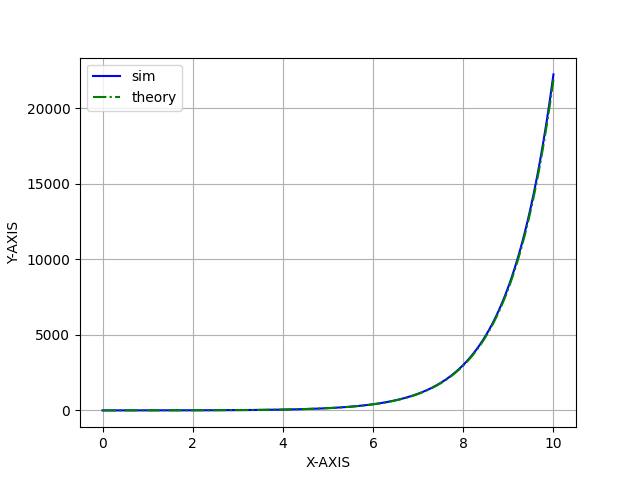
\includegraphics[width=0.8\textwidth]{figs/fig.png}
				 \caption{A plot of the given question.}
				 \label{fig:Plot1}
			 \end{figure}


\end{document}
